\documentclass[12pt]{article}

\usepackage[a4paper,margin=2.5cm,footskip=0.7cm,headheight=1cm]{geometry}

\usepackage{mathtools}
\usepackage{amsmath}
\usepackage{scalerel,amssymb}
\usepackage{gensymb}
\usepackage{graphicx}
\usepackage{caption}
\usepackage{german}
\usepackage{tikz}

\newcommand{\overtext}[2]{\mathrel{\overset{\makebox[0pt]{\mbox{\normalfont\tiny\sffamily #2}}}{#1}}}
\newcommand{\comment}[1]{}
\DeclarePairedDelimiter\abs{\lvert}{\rvert}
\DeclarePairedDelimiter\brackets{(}{)}

%TODO
\title{\vspace{-2.0cm}Aufgabe 1}
\author{Nikolas Kilian}
\date{8. März 2019}

\usepackage{Csharp}
\usepackage{lastpage}
\usepackage{fancyhdr}
\pagestyle{fancy} 

\makeatletter
\let\runauthor\@author
\makeatother
\lhead{\runauthor}
\cfoot{\thepage\ von \pageref{LastPage}}

\begin{document}
\maketitle

\section{Lösungsidee}
Wenn es keine Hindernisse gibt, so ist der optimale Weg eine gerade Strecke vom Startpunkt zum Buspfad im 30\degree\ Winkel. Für Begründung davon siehe 1.1.\\
Gibt es Hindernisse, so ist der optimale Weg der optimale Weg zu einem Eckpunkt, von dem die 30\degree\ Strecke offen ist, und dann diese 30\degree\ Strecke.\\
Um das Optimum mit Hindernissen zu finden, muss man also alle Eckpunkte bestimmen, von denen aus diese 30\degree\ Strecke offen ist, und den optimalen Weg zu ihnen bestimmen. Da der optimale Weg das Format der resultierenden Wege hat, ist unter den resultierenden Wegen das Optimum enthalten, also muss man nun nur noch die Zeit, zu der Lisa loslaufen muss, für alle Wege errechnen und den Weg mit der spätesten Startzeit auswählen.
Der optimale Weg zu diesen Eckpunkten lässt sich bestimmen mithilfe eines Sichtbarkeitsgraphen und Dijkstra's Algorithmus. Zum verhindern von Strecken durch unendlich dünne Wege (berührende Polygone) veränderet man den Sichtbarkeitsgraphen, sodass für jede normal sichtbare Linie nachträglich auf unendlich dünne Wege geprüft werden.

\subsection{Berechnung}
\newcommand{\vb}{v_{Bus}}
\newcommand{\vl}{v_{Lisa}}

\newcommand{\x}{x}

\renewcommand{\a}{a}
\renewcommand{\b}{b}
\renewcommand{\c}{c}

\newcommand{\f}{f}
\newcommand{\fzero}{f_0}

\newcommand{\tf}{t(\f)}
\newcommand{\tfzero}{t(\fzero)}
\newcommand{\df}[1]{\frac{d#1}{d\f}}
\newcommand{\dtf}{\df{\tf}}
\newcommand{\dtfzero}{\df{\tfzero}}

\begin{minipage}{0.8\textwidth}
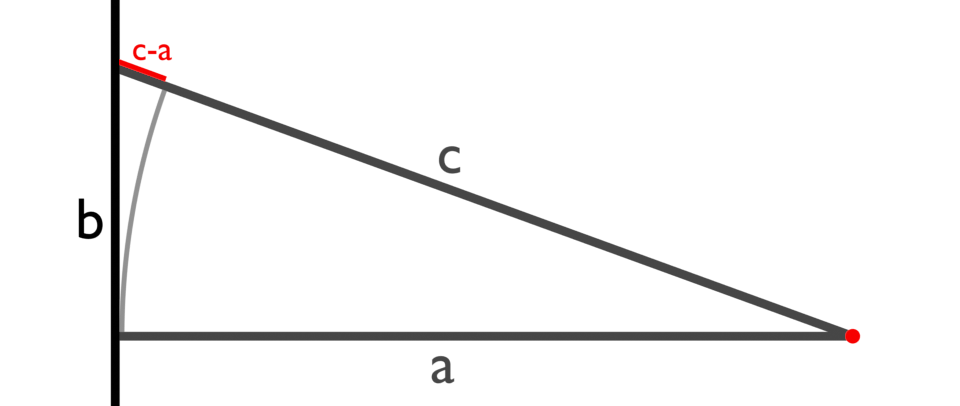
\includegraphics[scale=0.4]{CalcLabel}
\end{minipage}
\begin{minipage}{0.15\textwidth}
\vspace{-1cm}
\[\c=\sqrt{\a^2+\b^2}\]
\[\f:=\frac{\b}{\a}\]%\b=\a\f\]
\end{minipage}

\begin{minipage}{0.45\textwidth}
Der Zeitvorteil durch eine angewinkelte Strecke ist die Differenz zwischen der Zeit die Lisa braucht für ihre Extrastrecke, und die Zeit die der Bus mehr fährt.

\begin{align*}
\tf &= \frac{\c-\a}{\vl} - \frac{\b}{\vb}\\
&= \frac{\sqrt{\a^2+\b^2}-\a}{\vl} - \frac{\a\f}{\vb}\\
&= \frac{\sqrt{\a^2(1+\f^2)}-\a}{\vl} - \frac{\a\f}{\vb}\\
&= \a\left(\frac{\sqrt{1+\f^2}-1}{\vl} - \frac{\f}{\vb}\right)\\
\end{align*}
\end{minipage}
\begin{minipage}{0.55\textwidth}
\begin{align*}
\dtf &= \df{\a\left(\frac{\sqrt{1+\f^2}-1}{\vl} - \frac{\f}{\vb}\right)}\\
&= \a\left(\df{\frac{\sqrt{1+\f^2}-1}{\vl}} - \df{\frac{\f}{\vb}}\right)\\
&= \a\left(\frac{\df{\sqrt{1+\f^2}}}{\vl} - \frac{\df{\f}}{\vb}\right)\\
&= \a\left(\frac{\frac{1}{2\sqrt{1+\f^2}}\cdot\df{1+\f^2}}{\vl} - \frac{1}{\vb}\right)\\
&= \a\left(\frac{f}{\vl\sqrt{1+\f^2}} - \frac{1}{\vb}\right)\\
\end{align*}
\end{minipage}

Extremstellen dieser Zeitdifferenz stellen die besten und schlechtesten Winkel für Lisas Strecke da.
\begin{align*}
&&\dtfzero &= 0\\
\iff&&\a\left(\frac{\fzero}{\vl\sqrt{1+\fzero^2}} - \frac{1}{\vb}\right) &= 0\\
\iff&&\a\frac{\fzero}{\vl\sqrt{1+\fzero^2}} &= \a\frac{1}{\vb}\\
\iff&&\frac{\fzero}{\sqrt{1+\f^2}} &= \frac{\vl}{\vb}\\
\iff&&\left(\frac{\fzero}{\sqrt{1+\fzero^2}}\right)^2 &= \left(\frac{\vl}{\vb}\right)^2\\
\iff&&\frac{\fzero^2}{1+\fzero^2} &= \frac{\vl^2}{\vb^2}\\
\iff&&\frac{1+\fzero^2}{\fzero^2} &= \frac{\vb^2}{\vl^2}\\
\iff&&\frac{1}{\fzero^2} &= \frac{\vb^2-\vl^2}{\vl^2}\\
\iff&&\fzero^2 &= \frac{\vl^2}{\vb^2-\vl^2}\\
\iff&&\fzero &= \sqrt{\frac{\vl^2}{\vb^2-\vl^2}}\\
\iff&&\fzero &= \frac{\vl}{\sqrt{\vb^2-\vl^2}}\\
\end{align*}
Für die Standardwerte von Lisas Geschwindigkeit und der Busgeschwindigkeit, ist die Extremstelle $\fzero = \frac{1}{\sqrt{3}}$, wobei $\arctan(\fzero) = 30\degree$. Somit ist die optimale Strecke im 30\degree\ Winkel.

\section{Umsetzung}
Zur Umsetzung habe ich mich für eine Implementation in C\# entschieden, mit einer Visualisierung mithilfe von WPF.
Für die Generierung von Sichtbarkeitspolygonen verwende ich eine Implementation des Sweep-Line Algorithmus [Sources here]. Die Version des Algorithmus die ich verwende funktioniert wie folgt:
\begin{Csharp}
Let Intersections = Binary Search Tree, sorted by the order of intersection

foreach (Point p in Points sorted by their angle to Origin) {
	Intersections.RemoveAll(Connected Edges on Clockwise Side of p); 
	
	if (IsVisible(p)) VisibleVertices.Add(p);	
	
	Intersections.AddAll(Connected Edges on Counterclockwise Side of p);
}

boolean IsVisible(p) {
    if (!Origin.BetweenNeighbours(p) || !p.BetweenNeighbours(Origin)) return false;
    if (Origin and p are neighbours) return true;

    if (Intersections is not empty and its leftmost element intersects the line from Origin to Target) return false;
}
\end{Csharp}

\begin{minipage}{0.6\textwidth}
P.BetweenNeighbours(A) gibt dabei zurück, ob für einen Punkt P der Teil eines Polygons ist ob A in dem in Abb. 1 grün markiertem Bereich liegt. Ist das Polygon in P nicht konvex, so ist das Ergebnis immer false.

Wenn der Rückgabewert dieser Methode false ist, so sind in einem reduziertem Sichtbarkeitsgraph die beiden Punkte nicht verbunden.
\end{minipage}\hspace{0.5cm}
\begin{minipage}{0.35\textwidth}
\frame{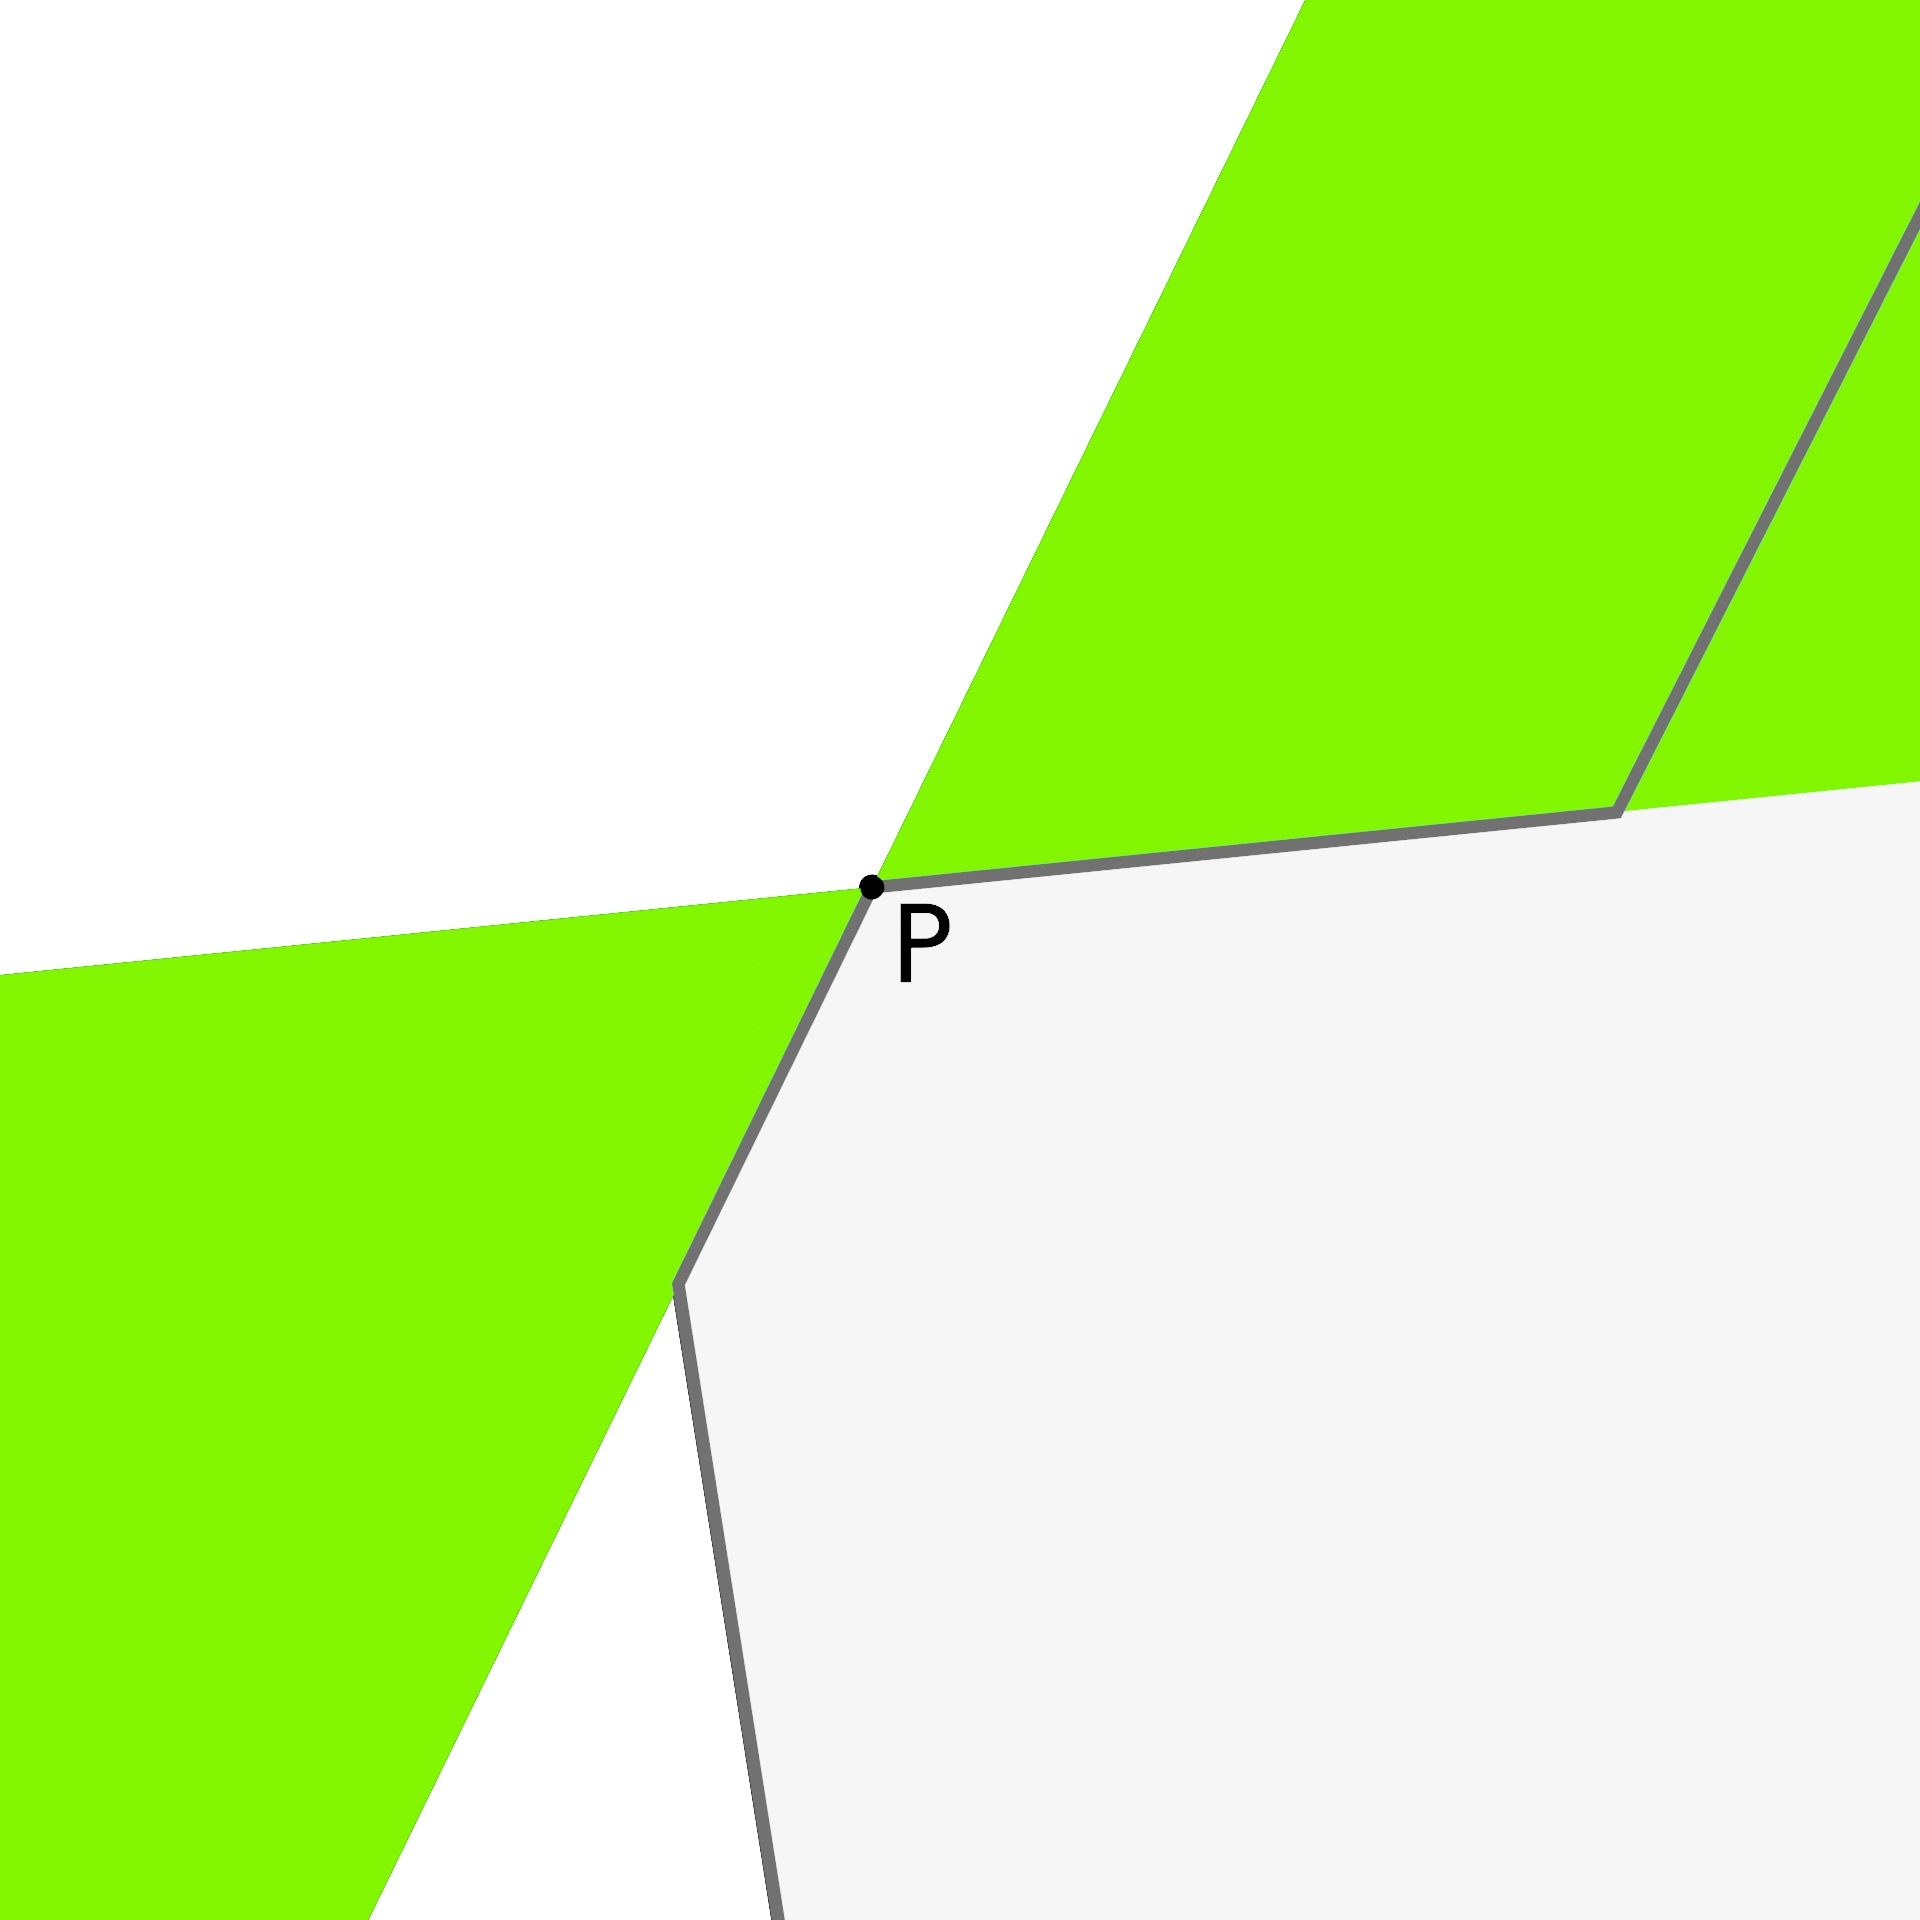
\includegraphics[scale=0.08]{Poly}}
\captionof{figure}{BetweenNeighbours}
\end{minipage}

Um das durchgehen unendlich dünner Wege zu verhindern, speichere ich die hinzugefügten/entfernten Kanten, errechne die Strecke die sie auf der Strecke zum aktuellem Punkt einnehmen, und errechne die Überschneidungen der linken und rechten Seite.

Um nun ein reduzierten Sichtbarkeitsgraphen zu generieren muss dieser Algorithmus nun nur noch für alle Punkte ausgeführt werden.

Mit dem Sichtbarkeitsgraphen fertig genreriere ich nun eine Heuristik mit Dijkstras Algorithmus, jedoch generiere ich diese nur bis allen Endpunkten (Enden der 30\degree\ Strecken, auf dem Buspfad) von Dijkstra besucht wurden (/an der Spitze der Priotitätsliste waren).

Da Dijkstra's Algorithmus nicht immer alle Knoten besucht, muss der Sichtbarkeitsgraph auch nicht vollständig generiert werden. Um dies auszunutzen berechne ich das Sichtbarkeitspolygon nur für Punkte die Dijkstra besucht.

Sobald die Heuristik fertig generiert ist, errechne mit dieser die optimale Strecke zu allen Endpunkten und die Zeit die Lisa braucht um diese abzulaufen, und die Zeit die der Bus braucht, um dorthin zu kommen. Damit errechne ich die Zeit zu der Lisa losgehen muss für alle diese Wege, vergleiche diese und nehme den Weg mit der spätesten Startezeit. Dieser Weg ist der optimale Weg, und somit das Ergebnis.

\newcommand{\ExNoPage}[3]{
\frame{\includegraphics[scale=#1]{#2}}
\captionof{figure}{#3}
}
\newcommand{\Ex}[3]{
\begin{minipage}{0.48\textwidth}
\ExNoPage{#1}{#2}{#3}
\end{minipage}
}

\section{Beispiele}
\subsection{Beispiel 1}
\begin{center}
\Ex{0.35}{Ex1Graph}{Sichtbarkeitsgraph}
\Ex{0.35}{Ex1Heuristic}{Dijkstra Heuristik}
\ExNoPage{0.7}{Ex1Result}{optimaler Weg}
\end{center}

\subsection{Beispiel 2}
\begin{center}
\Ex{0.45}{Ex2Graph}{Sichtbarkeitsgraph}
\Ex{0.45}{Ex2Heuristic}{Dijkstra Heuristik}
\ExNoPage{0.9}{Ex2Result}{optimaler Weg}
\end{center}

\subsection{Beispiel 3}
\begin{center}
\Ex{0.42}{Ex3Graph}{Sichtbarkeitsgraph}
\Ex{0.42}{Ex3Heuristic}{Dijkstra Heuristik}
\ExNoPage{0.85}{Ex3Result}{optimaler Weg}
\end{center}

\subsection{Beispiel 4}
\begin{center}
\Ex{0.44}{Ex4Graph}{Sichtbarkeitsgraph}
\Ex{0.44}{Ex4Heuristic}{Dijkstra Heuristik}
\ExNoPage{0.87}{Ex4Result}{optimaler Weg}
\end{center}

\subsection{Beispiel 5}
\begin{center}
\Ex{0.4}{Ex5Graph}{Sichtbarkeitsgraph}
\Ex{0.4}{Ex5Heuristic}{Dijkstra Heuristik}
\ExNoPage{0.74}{Ex5Result}{optimaler Weg}
\end{center}

\subsection{Beispiel 6}
\begin{center}
\Ex{0.45}{ExCGraph}{Sichtbarkeitsgraph}
\Ex{0.45}{ExCHeuristic}{Dijkstra Heuristik}
\Ex{0.45}{ExCResult}{optimaler Weg}\hspace{0.2cm}
\begin{minipage}{0.48\textwidth}
Dieses Beispiel ist eine Modifikation von Beispiel 5, bei der der Buspfad Um die Polygone herumgeht, und der Bus statt mit 30km/h mit 50km/h fährt.
In der Datei: 
\begin{Csharp}
// Normale Datei wie vorgegeben
// Buspfad angegeben wie Polygone, wobei inf und -inf positive und negative Unendlichkeit angeben
/*Lisas Geschwindigkeit in km/h*/ /*Busgeschwindigkeit in km/h*/
\end{Csharp}
\end{minipage}
\end{center}

\section{Code}

\begin{Csharp}[caption=Results]
List<Vertex> optimalPath = map.GetOptimalPath(out double characterLength, out double busLength, out double advantage, out var debug);
            
DateTime start = DateTime.Now.Let(x => new DateTime(x.Year, x.Month, x.Day, 7, 30, 0));

output.Text =
@$"Startzeit:{(start - TimeSpan.FromSeconds(advantage))}
Ankunft:{(start + TimeSpan.FromSeconds(busLength / map.busSpeed))}
Fahrzeit:{TimeSpan.FromSeconds(busLength / map.busSpeed)}
Laufzeit:{TimeSpan.FromSeconds(characterLength / map.characterSpeed)}
Weg:{string.Join("=>", Enumerable.Reverse(optimalPath).Select(x => $"({x.vector.x}, {x.vector.y})"))}";
\end{Csharp}

\begin{Csharp}[caption=class Polygon]
public Vertex[] vertices;
public int Length => vertices.Length;
public Vertex this[int index] => vertices[MathHelper.PositiveModulo(index, 0, Length)];

// Polygons are always sorted to be Counterclockwise
\end{Csharp}

\begin{Csharp}[caption=class Vertex]
public readonly Vector vector;
public readonly Polygon polygon;
public readonly int index;

public bool notConvex;

public Vertex Init()
{
    notConvex = Vector.Orientation(Previous.vector, vector, Next.vector) == Vector.VectorOrder.Clockwise; // Polygons are Counterclockwise
    return this;
}

public Vertex Previous => polygon[index - 1];
public Vertex Next => polygon[index + 1];

public bool IsNeighbor(Vertex other) => Previous == other || Next == other;

// Assumes notConvex to be properly calculated
public bool BetweenNeighbors(Vector other) =>
    !notConvex && (Vector.Orientation(vector, Previous.vector, other) != Vector.Orientation(Next.vector, vector, other));
\end{Csharp}

\begin{Csharp}[caption=class Vector]
public double x, y;

public Vector() { }

public Vector(double angle) : this(Math.Cos(angle), Math.Sin(angle)) { }

public Vector(double x, double y)
{
    this.x = x;
    this.y = y;
}

public Vector Left => new Vector(-y, x);
public Vector Right => new Vector(y, -x);
public Vector Back => new Vector(-x, -y);

// Algorithm from https://bryceboe.com/2006/10/23/line-segment-intersection-algorithm/
public enum VectorOrder : int
{
    Collinear = -1,
    Clockwise = 0,
    Counterclockwise = 1,
}
/// <summary>
/// Calculates the orientation of the triangle defined by a, b and c
/// </summary>
public static VectorOrder Orientation(Vector a, Vector b, Vector c)
{
    double orientation = (c.y - a.y) * (b.x - a.x) - (b.y - a.y) * (c.x - a.x);

    if (orientation <  0) return VectorOrder.Clockwise;
    if (orientation == 0) return VectorOrder.Collinear;
    if (orientation >  0) return VectorOrder.Counterclockwise;

    throw new NotFiniteNumberException();
}
/// <summary>
/// Like Orientation, but provides a margin for collinearity
/// </summary>
/// <param name="epsilon">The margin for collinearity</param>
public static VectorOrder OrientationApprox(Vector a, Vector b, Vector c, double epsilon)
{
    double orientation = (c.y - a.y) * (b.x - a.x) - (b.y - a.y) * (c.x - a.x);

    if (orientation < -epsilon) return VectorOrder.Clockwise;
    if (orientation > epsilon) return VectorOrder.Counterclockwise;

    if (double.IsNaN(orientation)) throw new NotFiniteNumberException();
    return VectorOrder.Collinear;
}
public static bool IntersectingLines(Vector startA, Vector endA, Vector startB, Vector endB)
{
    VectorOrder sAsBeB = Orientation(startA, startB, endB);
    VectorOrder eAsBeB = Orientation(endA, startB, endB);
    VectorOrder sAeAsB = Orientation(startA, endA, startB);
    VectorOrder sAeAeB = Orientation(startA, endA, endB);

    return (sAsBeB != eAsBeB && sAeAsB != sAeAeB)
            && !(sAeAeB == VectorOrder.Collinear || eAsBeB == VectorOrder.Collinear || sAeAsB == VectorOrder.Collinear || sAeAeB == VectorOrder.Collinear);
}
\end{Csharp}

\begin{Csharp}[caption=class Helper]
public static int PositiveModulo(int value, int offset, int length)
{
    while (value < offset) value += length;
    while (value >= offset + length) value -= length;
    return value;
}
public static double PositiveModulo(double value, double offset, double length)
{
    while (value < offset) value += length;
    while (value >= offset + length) value -= length;
    return value;
}
public static double ModuloAngle(double angle) => PositiveModulo(angle, 0, 2 * Math.PI);

public static double Clamp(double value, double min, double max) => value < min ? min : value > max ? max : value;

public static bool Approx(this double first, double second, double epsilon) => Math.Abs(first - second) < epsilon;
public static bool Approx(this Vector first, Vector second, double epsilonSquared) => first.DistanceSquared(second) < epsilonSquared;

public static (T1 value, T2 comparable) MinValue<T1, T2>(this IEnumerable<T1> enumerable, Func<T1, T2> selector) where T2 : IComparable<T2>
// Returns the element with the lowest return value selector(x) out of an enumerable, along with that return value
public static T MaxValue<T>(this IEnumerable<T> enumerable, Comparison<T> comparer)
// Returns the element with the highest element out of an enumerable, as defined by the given comparer

public static T2 Let<T1, T2>(this T1 obj, Func<T1, T2> func) => func(obj);
public static void Let<T>(this T obj, Action<T> action) => action(obj);
\end{Csharp}

\begin{Csharp}[caption=class Map]
public Polygon[] polygons;
public Vector[] busPath;
public Vertex startingPosition;
public List<Vertex> allPolygonVertices;
public double busSpeed, characterSpeed, busApproachConstant;

public void SetSpeed(double characterSpeed, double busSpeed)
{
    this.characterSpeed = characterSpeed;
    this.busSpeed = busSpeed;
    busApproachConstant = characterSpeed / Math.Sqrt(busSpeed * busSpeed - characterSpeed * characterSpeed);
}

public IEnumerable<Vector> GetEndpoints(Vector dot)
// Returns all endpoints of the direct paths (30 degree angle) from the given Vector to the bus path

public double CalculateDistanceAtAngle(Vertex vertex, Vector origin, double angle)
// Calculates the distance from origin to the intersection between a ray from origin with a given angle, and the line containing vertex and vertex.Next

public double epsilon = 1E-15;

public List<Vertex> GenerateVisibilityPolygon(Vertex originVertex, out List<(Vertex vert, double busLength)> endpoints, out List<(Vector, Vector)> debug)
{
    List<(Vector, Vector)> debugOut = new List<(Vector, Vector)>();

    Vector origin = originVertex.vector;

    List<Vertex> visibilityGraph = new List<Vertex>();
    List<Vertex> allPolygonVertices = this.allPolygonVertices.Where(x => !x.vector.Approx(origin, epsilon)).ToList();

    endpoints = GetEndpoints(origin).ToList();
    Dictionary<Vertex, double> angles =
        allPolygonVertices
        .Concat(endpoints.Select(x => x.Item1))
        .ToDictionary(x => x, x => x.vector.Angle(origin));

    // Edges are stored as the vertex with the lower index of the two defining vertices
    IComparer<Vertex> comparer = Comparer<Vertex>.Create((a, b) =>
    {
        if (ReferenceEquals(a, b) || a == b) return 0;

        // Based on https://github.com/trylock/visibility/blob/master/visibility/visibility.hpp Lines 17-89

        Vector a1 = a.vector;
        Vector a2 = a.Next.vector;
        Vector b1 = b.vector;
        Vector b2 = b.Next.vector;

        // If there are common endpoints, let them be a1 and b1
        if (a2.Approx(b1, epsilon) || a2.Approx(b2, epsilon)) (a1, a2) = (a2, a1);
        if (a1.Approx(b2, epsilon)) (b1, b2) = (b2, b1);

        if (a1.Approx(b1, epsilon)) // If there are common endpoints a1 and b1 this is true
        {
            if (a2.Approx(b2, epsilon)) return 0; // Same Lines
            // a and b are on opposing sides of ray from origin to shared point (current ray in sweep-line algorithm)
            if (Vector.OrientationApprox(origin, a1, b2, epsilon) != Vector.OrientationApprox(origin, a1, a2, epsilon)) 
            {
                throw new Exception("Attempted Change to early");
            }

            // b2 is on the same side of a as origin => b is below a
            return Vector.OrientationApprox(a1, a2, b2, epsilon) == Vector.OrientationApprox(a1, a2, origin, epsilon) ? 1 : -1; 
        }
        else
        {
            var ba1 = Vector.OrientationApprox(b1, b2, a1, epsilon);
            var ba2 = Vector.OrientationApprox(b1, b2, a2, epsilon);

            // Line Segments are on a shared line but don't have common endpoints 
            if (ba2 == Vector.VectorOrder.Collinear && ba1 == Vector.VectorOrder.Collinear)
            { 
                // Since the line segments are on a shared line, only one point needs to be compared
                return origin.DistanceSquared(a1).CompareTo(origin.DistanceSquared(b1));
            }
            else if (ba1 == ba2 // a1 and a2 are entirely above or below b
                    || ba1 == Vector.VectorOrder.Collinear || ba2 == Vector.VectorOrder.Collinear) // or a has one point on b => a is entirely above or below b
            { 
                var bOrigin = Vector.OrientationApprox(b1, b2, origin, epsilon);
                return bOrigin == ba1 // a1 is on the same side of b as origin => a is closer 
                    || bOrigin == ba2 // a2 is on the same side of b as origin => a is closer // Check both as one might be collinear
                    ? -1 : 1;
            }
            else // a1 and a2 are on opposing sides of b (a crosses the infinite line containing b) => b is entirely above or below a
            {
                return Vector.OrientationApprox(a1, a2, origin, epsilon) == Vector.OrientationApprox(a1, a2, b1, epsilon) // b1 is on the same side of a as origin => b is below a
                        ? 1 : -1;
            }
        }
    });
    SortedSet<Vertex> intersections = new SortedSet<Vertex>(comparer);

    foreach (Vertex polygonVertex in allPolygonVertices)
    {
        if ((polygonVertex.Next.vector - origin).y * (polygonVertex.vector - origin).y < -epsilon
            && CalculateDistanceAtAngle(polygonVertex, origin, 0) >= epsilon)
        {
            intersections.Add(polygonVertex);
        }
    }

    List<(double min, double max)> leftTouching = new List<(double, double)>();
    List<(double min, double max)> rightTouching = new List<(double, double)>();

    List<(double min, double max)> GetLeft() => leftTouching;
    List<(double min, double max)> GetRight() => rightTouching;

    bool IsVisible(Vertex target)
    {
        if (!(target.polygon is null))
        {
            if (!target.BetweenNeighbors(origin)) return false;
        }
        if (!(originVertex.polygon is null))
        {
            if (!originVertex.BetweenNeighbors(target.vector)) return false;
            if (originVertex.IsNeighbor(target)) return true; // Neighbours are not always visible in a reduced graph
        }

        if (intersections.Count != 0 &&
            intersections.First().Let(x => Vector.IntersectingLines(origin, target.vector, x.vector, x.Next.vector))) return false;

        var furthestDistance =
            GetLeft()
            .SelectMany(x => GetRight()
                .Where(y =>
                    (x.min <= y.min && y.min <= x.max)
                    || (x.min <= y.max && y.max <= x.max)
                ) // Only take intersections
                .Select(y => Math.Max(x.min, y.min))
            )
            .Let(blocked => blocked.Any() ? blocked.Min() : double.PositiveInfinity);

        if (origin.Distance(target.vector) > furthestDistance) return false;

        return true;
    }

    (Vertex vert, double currentAngle)[] sortedAngles = angles
        .Select(x => (x.Key, x.Value)).ToArray();
    Array.Sort(sortedAngles, Comparer<(Vertex vert, double currentAngle)>.Create((a, b) => a.currentAngle.CompareTo(b.currentAngle)));
    IEnumerable<(Vertex vert, double currentAngle)> sortedAnglesEnum = sortedAngles;

    // Group vertices with the same angle together
    var vertsByAngle = new List<(List<Vertex> vertices, double prevAngle, double angle, double nextAngle)>();
    {
        double angle;
        double prevAngle = 0;
        while (sortedAnglesEnum.Any())
        {
            angle = sortedAnglesEnum.First().currentAngle;
            List<Vertex> buffer = sortedAnglesEnum.TakeWhile(x => x.currentAngle == angle).Select(x => x.vert).ToList();
            sortedAnglesEnum = sortedAnglesEnum.Skip(buffer.Count);
            vertsByAngle.Add((buffer, prevAngle, angle, sortedAnglesEnum.Any() ? sortedAnglesEnum.First().currentAngle : Math.PI * 2));
            prevAngle = angle;
        }
    }

    List<Vertex> delta = new List<Vertex>();

    void Add(double currentAngle, double nextAngle, Vertex first, Vertex second)
    {
        if (first.vector.Approx(origin, epsilon) || second.vector.Approx(origin, epsilon)) return; // Already handeled by BetweenNeighbours

        // Collinear lines aren't intersections, only their position on the ray is used
        if (Vector.OrientationApprox(origin, first.vector, second.vector, epsilon) != Vector.VectorOrder.Collinear) delta.Add(first);
        leftTouching.Add(angles[first] == angles[second]
                ? (origin.DistanceSquared(first.vector), origin.DistanceSquared(second.vector)) // Squaring later is cheaper than Sqrt here
                    .Let(x => x.Item1 < x.Item2 ? x : (x.Item2, x.Item1))
                : origin.DistanceSquared(first.vector).Let(x => (x, x)));
    }
    void Remove(double prevAngle, double currentAngle, Vertex first, Vertex second)
    {
        if (first.vector.Approx(origin, epsilon) || second.vector.Approx(origin, epsilon)) return; // Already handeled by BetweenNeighbours

        // Collinear lines aren't intersections, only their position on the ray is used
        if (Vector.OrientationApprox(origin, first.vector, second.vector, epsilon) != Vector.VectorOrder.Collinear) intersections.Remove(first);
        rightTouching.Add(angles[first] == angles[second]
                ? (origin.DistanceSquared(first.vector), origin.DistanceSquared(second.vector)) // Squaring later is cheaper than Sqrt here
                    .Let(x => x.Item1 < x.Item2 ? x : (x.Item2, x.Item1))
                : origin.DistanceSquared(first.vector).Let(x => (x, x)));
    }

    foreach ((List<Vertex> vertices, double prevAngle, double currentAngle, double nextAngle) in vertsByAngle)
    {
        foreach (Vertex vert in vertices)
        {
            if (vert.polygon is null) continue;

            Vertex previous = vert.Previous;
            if (Vector.Orientation(previous.vector, vert.vector, origin) != Vector.VectorOrder.Clockwise) Remove(prevAngle, currentAngle, previous, vert);
            else Add(currentAngle, nextAngle, previous, vert);

            Vertex next = vert.Next;
            if (Vector.Orientation(next.vector, vert.vector, origin) != Vector.VectorOrder.Clockwise) Remove(prevAngle, currentAngle, vert, next);
            else Add(currentAngle, nextAngle, vert, next);
        }

        visibilityGraph.AddRange(vertices.Where(IsVisible));

        leftTouching.Clear();
        rightTouching.Clear();

        delta.ForEach(x => intersections.Add(x));
        delta.Clear();
    }

    var polygon = visibilityGraph.Distinct().ToList();
    debug = debugOut;
    return polygon;
}

public Dictionary<Vertex, List<Vertex>> GenerateVisibilityGraph(out List<(Vertex vert, double busLength)> endpoints, out List<(Vector, Vector)> debug)
{
    var debugOut = new List<(Vector, Vector)>();
    var endpointsOut = new List<(Vertex vert, double busLength)>();
    var graph =
        allPolygonVertices
        .Concat(new[] { startingPosition })
        .ToDictionary(x => x, x =>
        {
            var polygon = GenerateVisibilityPolygon(x, out var newEndpoints, out var newDebug);
            debugOut.AddRange(newDebug);
            endpointsOut.AddRange(newEndpoints);
            return polygon;
        });

    debug = debugOut;
    endpoints = endpointsOut;
    return graph;
}

public Dictionary<Vertex, Vertex> GenerateDijkstraHeuristic(bool reduced, out Dictionary<Vertex, Dictionary<Vertex, double>> visitedNodes, out List<(Vertex vert, double busLength)> endpoints, out List<(Vector, Vector)> debug)
{
    List<Vertex> allVertices = allPolygonVertices.Concat(new[] { startingPosition }).ToList();

    var debugOut = new List<(Vector, Vector)>();
    var endpointsOut = new List<(Vertex vert, double busLength)>();

    Dictionary<Vertex, Func<Dictionary<Vertex, double>>> graph =
        allVertices.ToDictionary(x => x, x =>
        (Func<Dictionary<Vertex, double>>)(() =>
            {
                var polygon = GenerateVisibilityPolygon(x, out var newEndpoints, out var newDebug);
                debugOut.AddRange(newDebug);
                endpointsOut.AddRange(newEndpoints);
                return polygon.ToDictionary(y => y, y => y.vector.Distance(x.vector));
            }
        ));

    var dijkstra = Dijkstra.GenerateDijkstraHeuristicLazy(startingPosition, graph, endpointsOut.Select(x => x.vert).ToList(), out visitedNodes);
    debug = debugOut;
    endpoints = endpointsOut;
    return dijkstra;
}

public List<Vertex> GetOptimalPath(out double characterLength, out double busLength, out double advantage, out List<(Vector, Vector)> debug)
{
    var heuristic = GenerateDijkstraHeuristic(true, out var visitedNodes, out var endpoints, out debug);

    IEnumerable<(Vertex vert, double characterLength, double busLength)> times = endpoints
        .Where(x => heuristic.ContainsKey(x.vert))
        .Select(x => 
            (x.vert, Dijkstra.GetPathLength(startingPosition, x.vert, heuristic, visitedNodes), x.busLength));

    Vertex min;
    ((min, characterLength, busLength), advantage) = times.MinValue(x => x.characterLength / characterSpeed - x.busLength / busSpeed);
    return Dijkstra.GetPath(startingPosition, min, heuristic);
}
\end{Csharp}

\begin{Csharp}[caption=class Dijkstra]
public static Dictionary<Vertex, Vertex> GenerateDijkstraHeuristicLazy(Vertex start, Dictionary<Vertex, Func<Dictionary<Vertex, double>>> nodes, List<Vertex> reachingRequired, out Dictionary<Vertex, Dictionary<Vertex, double>> visitedNodes)
{
    List<Vertex> priorityList = nodes.Keys.ToList();
    reachingRequired = reachingRequired.Where(x => priorityList.Contains(x)).ToList();

    Dictionary<Vertex, double> distance = new Dictionary<Vertex, double>();
    Dictionary<Vertex, Vertex> path = new Dictionary<Vertex, Vertex>();
    Dictionary<Vertex, Dictionary<Vertex, double>> visitedNodesOut = new Dictionary<Vertex, Dictionary<Vertex, double>>();
    distance[start] = 0;
    path[start] = start;

    void Step(Vertex current)
    {
        foreach (var connection in (visitedNodesOut[current] = nodes[current]()))
        {
            double newDistance = connection.Value + distance[current];
            if (!distance.ContainsKey(connection.Key)) distance[connection.Key] = double.PositiveInfinity;
            if (distance[connection.Key] > newDistance)
            {
                path[connection.Key] = current;
                distance[connection.Key] = newDistance;
            }
        }

        priorityList.Remove(current);
        reachingRequired.Remove(current);
    }
    IComparer<Vertex> comparer = Comparer<Vertex>.Create((a, b) => distance[a].CompareTo(distance[b]));
    while (priorityList.Any()) Step(priorityList.MinValue(x => distance.ContainsKey(x) ? distance[x] : double.PositiveInfinity).value);

    visitedNodes = visitedNodesOut;
    return path.ToDictionary(x => x.Key, x => x.Value);
}

public static List<Vertex> GetPath(Vertex start, Vertex end, Dictionary<Vertex, Vertex> heuristic)
{
    List<Vertex> path = new List<Vertex>();
    for (Vertex current = end, next = heuristic[end]; current != start; current = next, next = heuristic[current]) path.Add(current);
    path.Add(start);
    return path;
}

public static double GetPathLength(Vertex start, Vertex end, Dictionary<Vertex, Vertex> heuristic, Dictionary<Vertex, Dictionary<Vertex, double>> visitedNodes)
{
    double length = 0;
    for (Vertex current = end, next = heuristic[end]; current != start; current = next, next = heuristic[current]) length += visitedNodes[next][current];
    return length;
}
\end{Csharp}

\end{document}